\section{簡介}
本章節以及下一個章節將對於問答系統介紹。在過去,閱讀理解和問答系統已經有很多研究提出模型,如加入專注式機制(Attention Mechanism)或急躁機制(Impatient Mechanism)的模型 \cite{hermann2015teaching} ,試圖想要模仿人類的行為,能忽視其他不重要或無關的輸入,只選擇專注於和需求有關的輸入,此方法最早在視覺圖像領域所提出,目的是希望讓機器學到圖片中所應該專注的物件(Object)或位置,而其成效也已經在圖像領域和機器翻譯中得到證實,如 \cite{mnih2014recurrent} 和 \cite{bahdanau2014neural},另有加入了記憶(Memory)網路的 Memory Network \cite{weston2014memory} ,可以儲存理解之後的資訊,概念如同 RNN cell 一般,還有端對端記憶網路(End to End Memory Network)\cite{sukhbaatar2015end} ,透過使用跳躍式(Hop)的機制,來多次更新記憶。本篇論文使用了專注式機制,來選擇文本的哪些部分該注意,使用記憶網路來儲存相關的文本,並且透過跳躍式機制來不斷更新記憶網路。

我們可將整個問答系統分成三個部分,首先針對使用者的查詢詞,透過檢索的方式回傳符合查詢詞的文本,但由於回傳的文本過多,因此我們需要一個過濾器(Filter)來判別此文本是否有此查詢詞之答案,以便降低文本的數量。最後在將這些被選出文本與其查詢詞,通過專注式記憶編碼解碼器(Attention-based Memory RNN Encoder-Decoder)\cite{xiong2016dynamic} 抽取出可能的答案,進而回傳給使用者。本論文之研究的檢索部分是採用 Bing 搜尋來取得相關之文本,故僅針對過濾器以及專注式記憶編碼解碼器兩者進行詳細介紹。

在詳細描述模型以前,我們將先簡介機器閱讀理解數據集。 Microsoft 釋出了閱讀理解相關的數據集,而以問答系統來實踐閱讀理解的概念。此數據集約莫有 10 萬筆的問答句以及約 20 萬以上的文章數,對於每個問句,都會有標註此問句的種類,如: cost to get a patent 是被分類為數值(Numeric)、 was ronald reagan a democrat 則是歸類成描述(Description)、diseases caused by clostridium 被歸為名詞(entity)、who was the president who caused the trail of tears 是為人物(Person),而 what sea is iceland in 則為地點(Location)等 5 類,表(\ref{table:query_percentage})和表(\ref{table:query_type})為機器閱讀理解查詢詞之比例。而 Bing 搜尋針對此問句,會提供大約 8 到 10 個左右的文本段落(Passages),人們再根據這些段落,標註此段落「是否」足夠提供問句之答案,並根據段落給予對應一至多個對應的答案。

\begin{table}
    \caption{問句包含詞比例}
    \label{table:query_percentage}
    \centering
    \begin{tabular}[h]{|l|l|}
        \hline
        問句包含詞  &百分比\\
        \hline
        what        &42.2\%\\
        \hline
        how         &15.3\%\\
        \hline
        where       &4.4\%\\
        \hline
        when        &2.0\%\\
        \hline
        why         &1.8\%\\
        \hline
        who         &1.7\%\\
        \hline
        which       &1.4\%\\
        \hline
    \end{tabular}
\end{table}
\begin{table}
    \caption{答案種類}
    \label{table:query_type}
    \centering
    \begin{tabular}{|l|l|}
        \hline
        問句類型            &百分比\\
        \hline
        描述(Description) &52.6\%\\
        \hline
        數字(Numberic)    &28.4\%\\
        \hline
        名詞(Entity)      &10.5\%\\
        \hline
        地點(Location)    &5.7\%\\
        \hline
        人物(Person)      &2.7\%\\
        \hline
    \end{tabular}
\end{table}

\section{模型架構介紹}
%\subsection{專注式記憶編碼解碼器}
圖 \ref{fig:dmn} 為本章節之系統架構圖之一。以下會針對此架構圖做分析。

\subsubsection{位置編碼}
首先每個段落透過 Natural Language Toolkit (NLTK)來做英文句子的斷句,即會得到 $M$ 個句子,每個詞都有一個詞向量 $w_j^i$,其中 $i$ 代表第 $i$ 個句子,而 $j$ 代表第 $i$ 個句子的第 $j$ 個詞,一個句子可以使用 RNN ,或者是詞袋模型(Bag of Word Model, BOW)來將編碼(Encode)成一個句向量(Sentence Vector),而此處則是採用位置編碼(Position Encoding)\cite{sukhbaatar2015end}  ,如式子(\ref{PE}),此處使用位置編碼的原因,一方面若是使用詞袋模型,會少了每個詞在句子上順序的重要性,另一方面,使用 RNN 模型雖然能夠有順序之別,但由於本篇論文模型過於複雜,若是使用 RNN 模型,將會有兩層 RNN 來處理詞彙與句子,因此會容易過度貼合,因此本篇論文採取折衷的方法,是採用位置編碼,可以得到每個句子的句向量 $f_i$ 代表第 $i$ 個句子

\begin{equation}
    f_i = \sum_{j=1}^M l_j \circ w_j^i
\end{equation}
其中 $\circ$ 為逐點乘積,而 $l_j$ 則為
\begin{equation}
    l_{jd} = (1 - \frac{j}{M}) - (\frac{d}{D})(1 - \frac{2j}{M}) \label{PE}
\end{equation}
其中 $d$ 是詞向量的第 $d$ 維, $D$ 是詞向量的維度,$j$ 代表一句話的第 $j$ 個詞。

\begin{figure}[h]
    \centering
    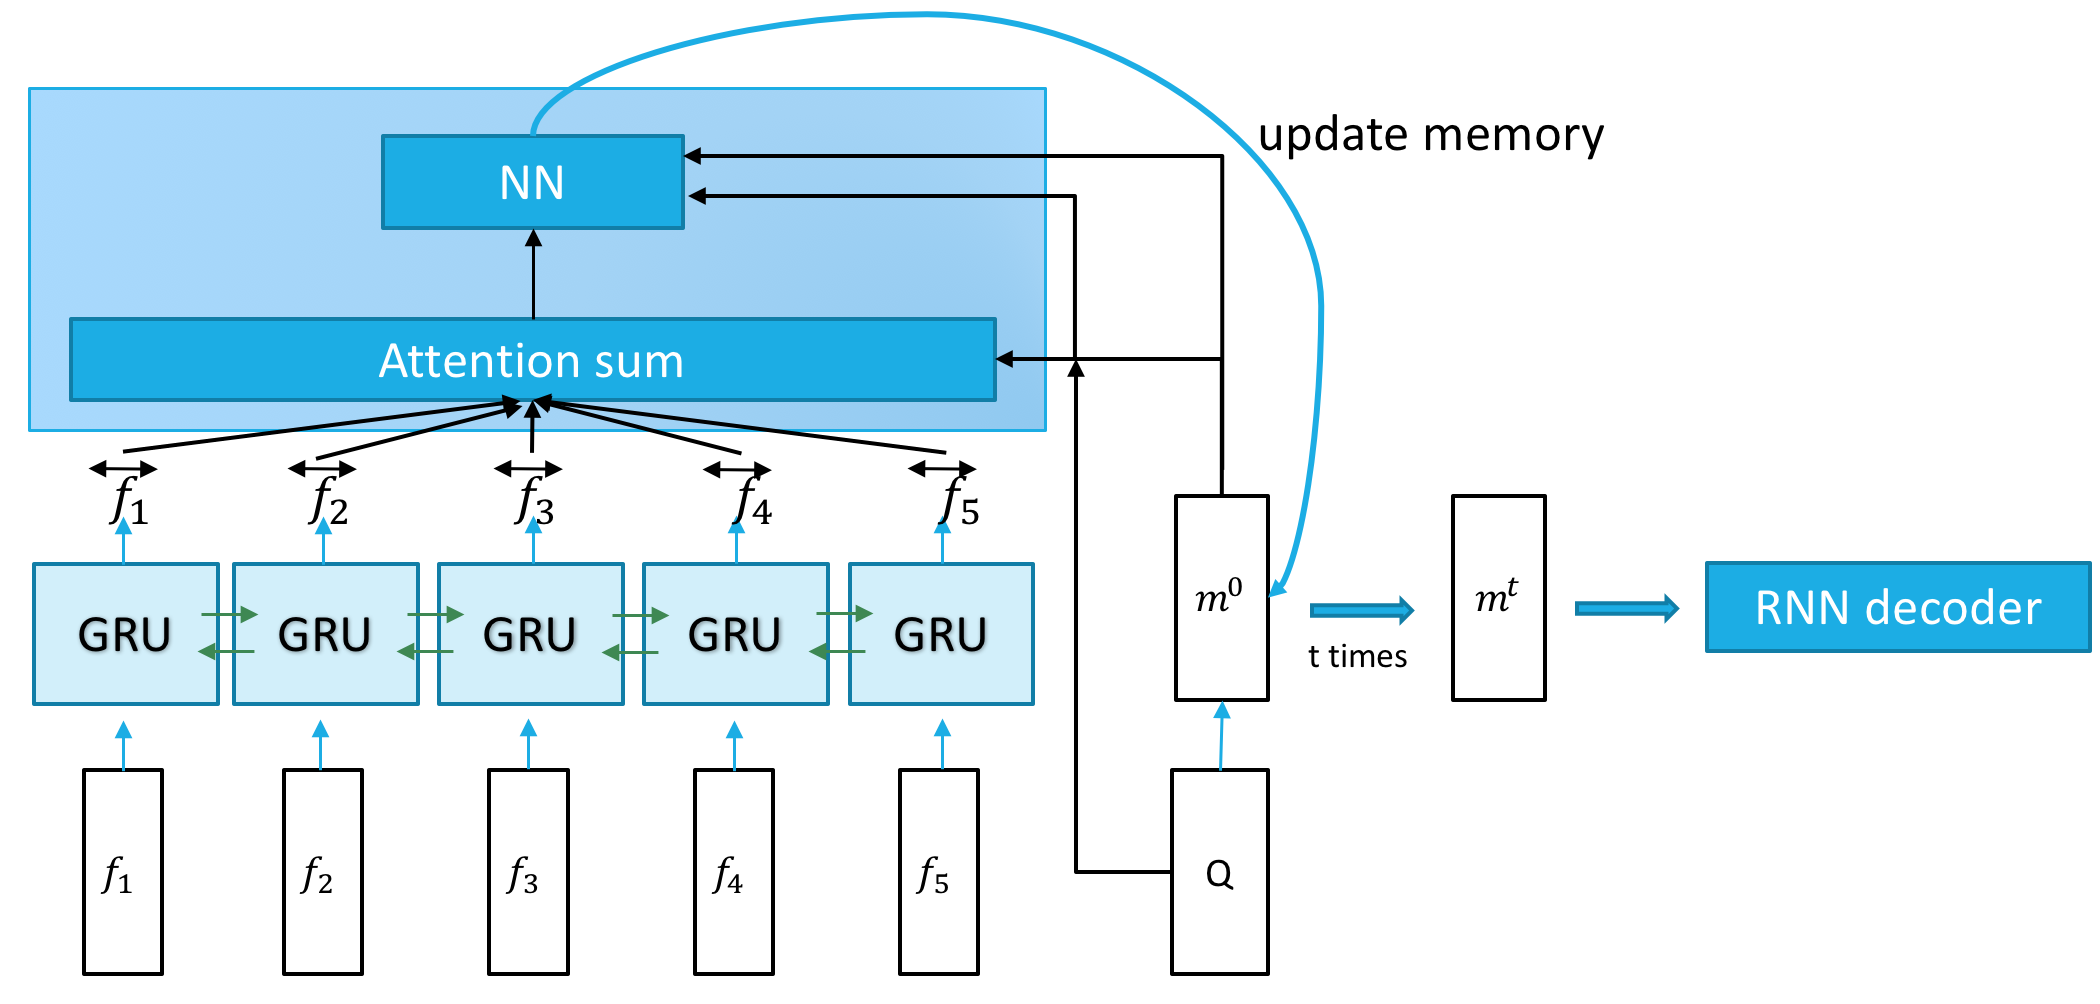
\includegraphics[scale=0.54]{images/chap3_dmn.png}
    \caption{專注式記憶編碼解碼器}\label{fig:dmn}
\end{figure}
\subsubsection{雙向式遞迴式類神經網路}
在得到句向量 $f_i$ 後,為了強化句子與句子彼此之間的關聯性,我們採取了雙向式遞迴式類神經網路(Bidirectional Recurrent Neural Network, BRNN),是由兩個遞迴式類神經網路,一為正向(Forward)遞迴式類神經網路輸出向量表示 $\overrightarrow{f_i}$ ,另一為反向(Backward)遞迴式類神經網路輸出向量表示 $\overleftarrow{f_i}$ ,並且取正向遞迴式類神經網路的第 $i$ 個時間點輸出向量 $\overrightarrow{f_i}$ ,與反向遞迴式類神經網路的第 $i$ 個時間點 $\overleftarrow{f_{M-i}}$ ,並把他們相加起來作為每個句子的向量表示 $\overleftrightarrow{f_i} = \overrightarrow{f_i} + \overleftarrow{f_i}$ ,即為圖 \ref{fig:dmn} 中 GRU 之輸出。雖然採取了雙向式遞迴式類神經網路,但依然容易失去長期的資訊,且我們不僅僅只是要讀過文本而已,我們更需要結合查詢詞來回答問題,因此在此處我們導入了專注式機制(Attention Mechanism)的技術。

\subsubsection{專注式機制}
專注式的機制,就是為了比較查詢詞 $Q$ 與文本 $\overleftrightarrow{f_i}$ 之間的相關性,然而專注式機制的實作方法有很多,但核心的概念是為了找尋兩者間之相似性(Similarity),即稱為專注式權重 $\alpha_i$ ,以下是幾種常見計算專注式權重之方法:
\itemsep -4pt
\begin{itemize}
    \item 歐式距離:$\alpha_i = ||Q-\overleftrightarrow{f_i}||_{2}$
    \item 餘弦相似性:
            $\alpha_i = \frac{Q \circ \overleftrightarrow{f_i} }{|Q| |\overleftrightarrow{f_i}| } $ 其中 $\circ$ 為 逐點乘積
    \item 類神經網路: $\alpha_i = W_a ([Q ; \overleftrightarrow{f_i}]) $ 
        ,其中 $\alpha_i$ 為一純量(Scalar) $;$ 代表串連兩個向量。
\end{itemize}
本論文採取最後一種深度類神經網路的方法,然此處深度神經網路的輸入是為 $z_i$ ,結合句子 $\overleftrightarrow{f_i}$ 、問句 $Q$ 以及記憶 $m$ 表示的資訊,如式子($\ref{function:nninput}$)
\begin{equation}
    z_i = [ \overleftrightarrow{f_i} \circ Q ; \overleftrightarrow{f_i} \circ m ; |\overleftrightarrow{f_i} - Q| ; | \overleftrightarrow{f_i} - m| ] \label{function:nninput}
\end{equation}
其中 $m$ 是經由 $Q$ 來初始化,而 $|\cdot|$ 是向量取絕對值。

接著讓 $z_i$ 通過兩層類神經網路,可得一純量 $Z_i$。在得到了專注式權重 $Z_i$ 以後,我們對其做正規化,此處我們選擇「對所有句子的 $\alpha$ 值通過軟性最大化」,透過軟性最大化可以更加強化相關的句子,降低其餘句子的雜訊,如式子($\ref{function:attention}$)
\begin{equation}
    g_i = \frac{exp{(Z_i)}}{\sum_{k=1}^{M} exp(Z_i)} \label{function:attention}
\end{equation}

結合正規化後的專注式權重 $g_i$ ,我們可對於文章抽取出基於我們想要專注點的語境向量(Contextual Vector),如式子(\ref{function:context_vector})
\begin{equation}
    c = \sum_{i=1}^{M} g_i \overleftrightarrow{f_i} \label{function:context_vector}
\end{equation}
%在得到了專注式權重以後,我們需要對其做正規化,
%而本篇論文另外使用了一種計算相似性的方法,
%\itemsep -2pt
%\begin{itemize}
%    \item Stochastic "Hard" Attention
%    \item Deterministic "Soft" Attention
%\end{itemize}
\subsubsection{記憶(Memory)}
下一步則是要更新記憶 $m$ ,一樣透過一個類神經網路,輸入為當前的記憶、語境向量、以及固定的問句表示,進而更新記憶,如式子(\ref{function:update_memory})
\begin{equation}
    m = ReLU(W [m; c; Q] +b) \label{function:update_memory}
\end{equation}
\subsubsection{跳躍式機制}
在此,我們把計算專注式權重的值以及新記憶的值,視為一個循環,我們把它稱為一個跳躍,每經過一次跳躍,相當於是再次讀過句子,重新理解再存入記憶裡。
\section{基本實驗配置}
\subsection{前置處理}
\itemsep -4pt
\begin{itemize}
    \item 前處理:此數據集包含大量的英文,夾雜部分日文以及標點符號,若是選用所有的詞彙(Vocabulary),會有四十幾萬的詞(Word),我們試著降低詞彙的數量,移除掉標點符號和文本中的網址,並把所有英文字母轉成小寫,最後我們把詞彙量降到了約莫 14 萬個詞。另外,為了再降低複雜度,我們特別對阿拉伯數字進行處理,把所有阿拉伯數字取代成特定標籤,或者是以文本數字出現的順序,分別給予數字一、數字二、數字三等等,把詞彙量降低到 13 萬左右。
    \item 訓練方法:我們選擇將詞嵌入一併與我們的模型一起訓練。而為了避免過度貼合,對於所有的遞迴式類神經網路,都使用了丟棄演算法,而對於所有的可訓練的(Trainable)權重進行正規化。在回顧機制裡,我們設置回顧次數的範圍在 1 到 3 次。此外我們採用 Negative Sampling 的技巧,來降低整個模型所需要的參數量
%TODO negative sampling
\end{itemize}
\subsection{基準實驗}
\begin{figure}[h]
    \centering
    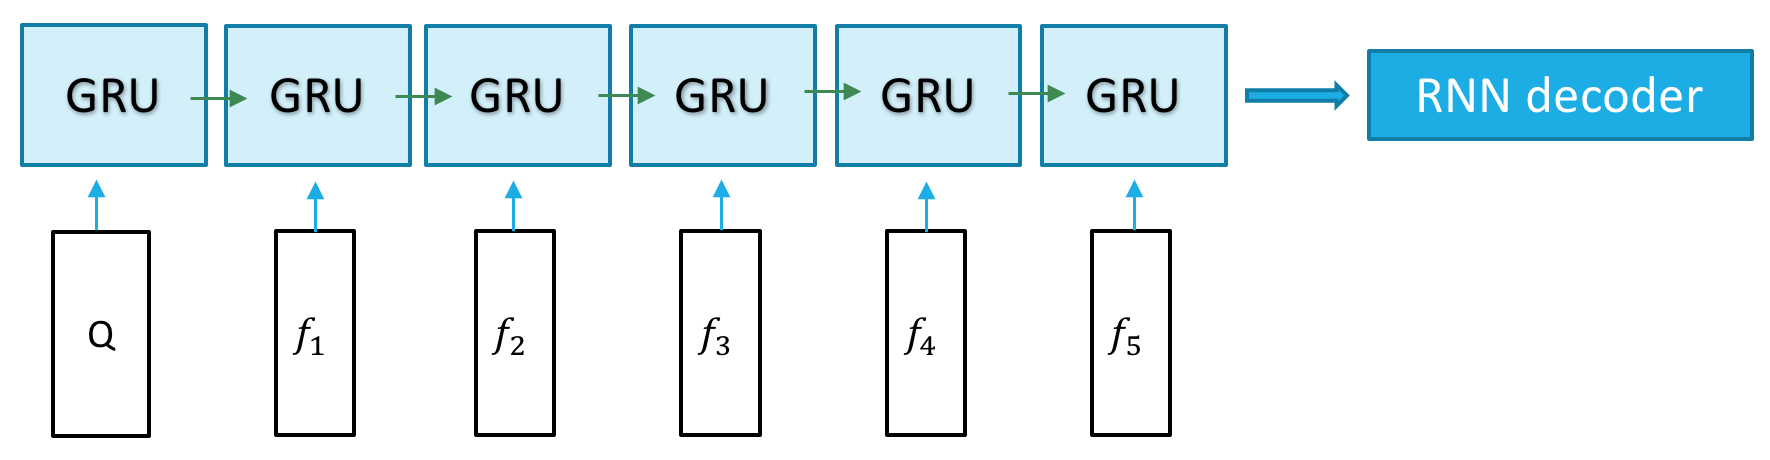
\includegraphics[scale=0.54]{images/chap3_baseline1.png}
    \caption{基準實驗模型一}\label{fig:baseline1}
\end{figure}
\begin{figure}[h]
    \centering
    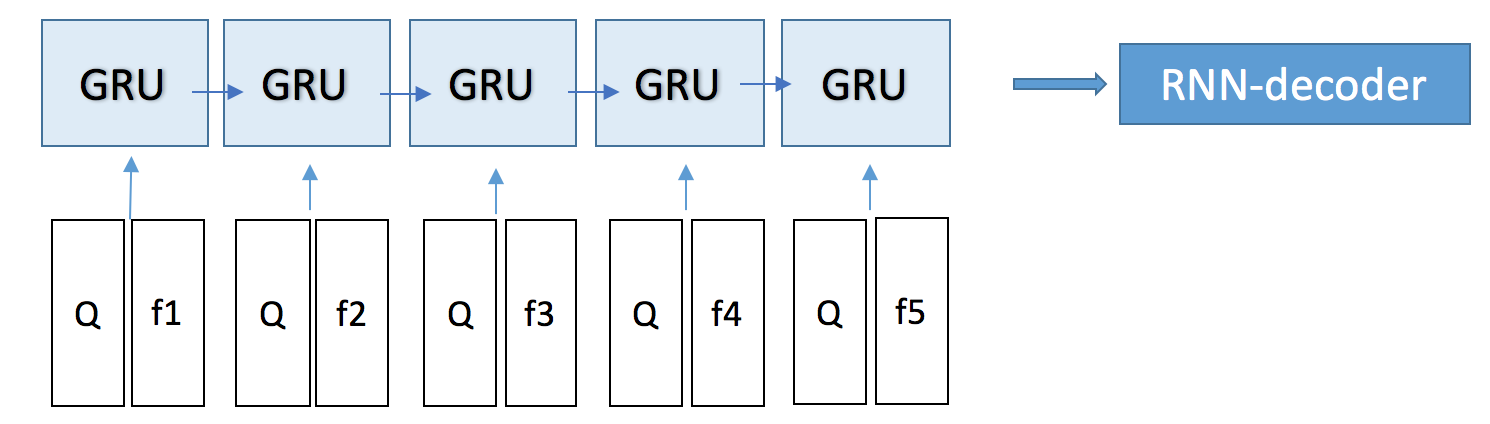
\includegraphics[scale=0.54]{images/chap3_baseline2.png}
    \caption{基準實驗模型二}\label{fig:baseline2}
\end{figure}

\section{實驗結果與討論}
\subsection{RNN}
\subsection{取代數字}
\subsection{回顧次數}
\subsection{模型}
%\subsection{更新記憶方法}
\section{範例與分析}
專注式機制在不同回顧的次數所專注之表現
\section{本章總結}
%\subsubsection{模型介紹}
